\documentclass[a4paper,12pt]{article}
\usepackage[utf8]{inputenc}
\usepackage{algorithmic}
\usepackage{algorithm}
\usepackage{pst-plot}
\usepackage{graphicx}
\usepackage{endnotes}
\usepackage{graphics}
\usepackage{graphicx}
\usepackage{floatflt}
\usepackage{wrapfig}
\usepackage{amsfonts}
\usepackage{amsmath}
\usepackage{verbatim}
\usepackage{hyperref}
\usepackage{multirow}
\usepackage{pdflscape}
\usepackage{multicol}
\usepackage[bottom]{footmisc}

\usepackage{hyperref}
\hypersetup{pdfborder={0 0 0 0}}

\pdfpagewidth 210mm
\pdfpageheight 297mm 
\setlength\topmargin{0mm}
\setlength\headheight{0mm}
\setlength\headsep{0mm}
\setlength\textheight{250mm}	
\setlength\textwidth{159.2mm}
\setlength\oddsidemargin{0mm}
\setlength\evensidemargin{0mm}
\setlength\parindent{0mm}
\setlength\parskip{3mm}

\graphicspath{{./images/}}



%
% Title
%
\begin{document}
\begin{center}
	{\Large
	University of Tartu\\
	Faculty of Mathematics and Computer Science\\
	Institute of Computer Science\\}
	\vspace{6cm}
	{\Large Kristjan Korjus, Ilya Kuzovkin, Ardi Tampuu, Taivo Pungas}\\
	\vspace{1.0cm}
	{\Huge Replicating the Paper ``Playing Atari with Deep Reinforcement Learning"\textsuperscript{\Large{\cite{mnih2013playing}}}}\\
	\vspace{0.5cm}
	{\Large Technical Report}\\
	\vspace{1.0cm}
	{\large MTAT.03.291 Introduction to Computational Neuroscience}
	
\end{center}
\vspace{9cm}
\begin{center}
	{\large Tartu 2014}
\end{center}
\thispagestyle{empty}
\pagebreak



%
% Table of contents
%
\thispagestyle{empty}
\tableofcontents
\pagebreak



%
% Introduction
%
\section*{Introduction}
\addcontentsline{toc}{section}{Introduction}
In the recent years the popularity of the method called \emph{deep learning} [REF] has increased noticeably in the machine learning community. Deep leaning was successfully applied to speech regonition [REF], something else [REF] and something else [REF]. In all these studies the performance of the resulting system was better than other machine learning methods were able to achieve so far.

The core of deep learning method is an artificial neural network. One of the properties, which gives this family of learning algorithms a special place, is the ability to extract ``meaningful" (from the human perspective) \emph{concepts} from the data by combining the features based on the structure of the data. The extracted concepts sometimes have clear interpretation and that makes us feel as if machine indeed has \emph{learned} something. Here we step into the realm of artificial intelligence, the possibility of which never stops to fascinate our minds.

One of the recent works, which brings together deep learning and artificial intelligence is a paper ``Playing Atari with Deep Reinforcement Learning"\cite{mnih2013playing} published by DeepMind\footnote{\url{http://deepmind.com}} company. The paper describes a system, which combines deep learning methods and \emph{reinforcement learning} in order to create a system that is able to learn how to play simple computer games. It is worth mentioning that the system has access only to the visual information (screen of the game) and the scores. Based on these two inputs the system learns to understand which moves are good and which are bad depending on the situation on the screen. Notice that the human player uses exactly same information to evaluate his performance and adapt his playing strategy. The reported result shows that the system was able to master several different games and play some of them better than the human player.

This result can be seen as a step forward to the truly intelligent machines and thus it fascinates us. The goal of this project is to create an open-source analogue of such a system using the description provided in the paper.



%
% Bird-eye view
%
\pagebreak
\section{A bird's-eye view of the system}
Before we go into the details, let us describe the overall architecture of the system and show how the building blocks are put together. 

\subsection{The task}

The system receives a picture of a game screen (an example is shown in Figure \ref{fig:breakoutscreen}) and chooses an action to take. It then executes this action and is told whether the score increased, decreased or did not change. Based on this information and playing a large number of games, the system needs to learn to improve its performance in the game.

\begin{figure}[h]
\centering
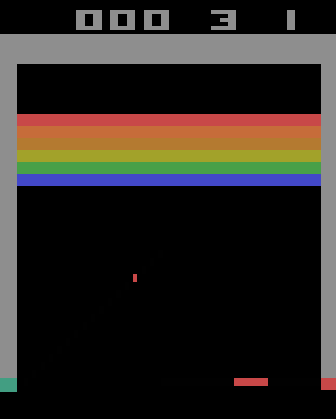
\includegraphics[width=3.5cm]{fig_gamescreen}
\caption{A game screen of Breakout.}
\label{fig:breakoutscreen}
\end{figure}

\subsection{Reinforcement learning}
This is a techinque... 

\subsubsection{Exploration-exploitation}
When the algorithm chooses between possible actions, it picks a "learned" action with probability $1-\epsilon$ and a random action with probability $\epsilon$. The value of $\epsilon$ is gradually decreased as the algorithm learns to play better.

[needs work]

multiarmed bandits

\subsection{Neural network}
The system uses a neural network to assign an expected reward value to each possible action. The input to the network at any time point consists of the last four preprocessed game screens the system received. This input is then passed through three successive hidden layers to the output layer. The output layer has one node for each possible action and the activation of those nodes indicates the expected reward from each of the possible actions.

\subsection{Learning process}
The system learns, i.e. improves the accuracy of its predictions, by updating the weights of connections between nodes in the neural network.

[needs expansion]

gradient descent blabla



%
% Components
%
\pagebreak
\section{Components of the system}
here goes the detailed description of everything (aka the hardest part)

\subsection{Convolutional neural network}
...

\subsection{Q-learning}
...

\subsection{Something else}
...


\subsection{And once again how all those things are put together}



%
% Implementation
%
\pagebreak
\section{Implementation details}
Programming language: Python 2.7 (32-bit).

Python libraries: Pillow, NumPy, Theano.

ATARI emulation environment: ALE (Arcade Learning Environement).

\subsection{Agent}
...

\subsection{Memory}
...

\subsection{Preprocessing}
\label{subsection_preproc}
The game screens are preprocessed by first cropping the original 160x210-pixel image to a 160x160 region of interest, which is then downscaled to a 84x84 image.

The colors from ATARI's NTSC palette are converted to RGB using a conversion table
\footnote{\url{http://www.biglist.com/lists/stella/archives/200109/msg00285.html}}. The RGB representation is then converted to grayscale according to the weighted combination $0.21R + 0.71G + 0.07B$. This should produce a representation close to human perception (humans are more sensitive to green than other colours)\footnote{\url{http://www.johndcook.com/blog/2009/08/24/algorithms-convert-color-grayscale/
}}. An example of a preprocessed image is shown in Figure \ref{fig:breakoutpreprocessed}.

\begin{figure}[h]
\centering

\includegraphics[width=2.5cm]{fig_preprocessedscreen}
\caption{A preprocessed game screen of Breakout.}
\label{fig:breakoutpreprocessed}
\end{figure}



\subsection{Any other implementational stuff which is worth describing}
...


%
% Results
%
\pagebreak
\section{Results}
Our system rules!

\subsection{Performance measures}

\subsection{Comparison to human player}
...

\subsection{Comparison to the paper}
...

\subsection{Something else}
...

\subsection{Applications and future blah}
...



%
% Appendicies
%
\pagebreak
\section*{Appendix A: Running instructions}
\addcontentsline{toc}{section}{Appendix A: Running instructions}
to test the system you should do this and that

you will see that blabla

this will make you happy

also go to github read wiki/code there for more details



%
% Bibliography
%
\pagebreak
\addcontentsline{toc}{section}{Bibliography}
\bibliographystyle{alpha}
\bibliography{report}

\end{document}